Web Browser haben sich seit der Veröffentlichung von Mosaic, einer der ersten populären Browser, im Jahr 1993 stark weiterentwickelt. Das Abrufen und Anzeigen von statischen HTML-Dokumenten wurde mit Hilfe von JavaScript um interaktive und später dynamische Inhalte erweitert. Heutzutage können in Browsern komplexe Webapplikationen realisiert werden, welche zudem unabhängig von einem speziellen Browser entwickelt werden können. Durch diese Entwicklung und die breiten Anwendungsfälle, besitzt die Umgebung ``Browser`` besondere Eigenschaften, welche nachfolgend beschrieben werden.

\subsection{Browserprodukte}
\label{sec:browserprodukte}

\begin{wrapfigure}[19]{r}{0.45\textwidth}
\centering
\tikzsetnextfilename{cross-browser_metastudie}
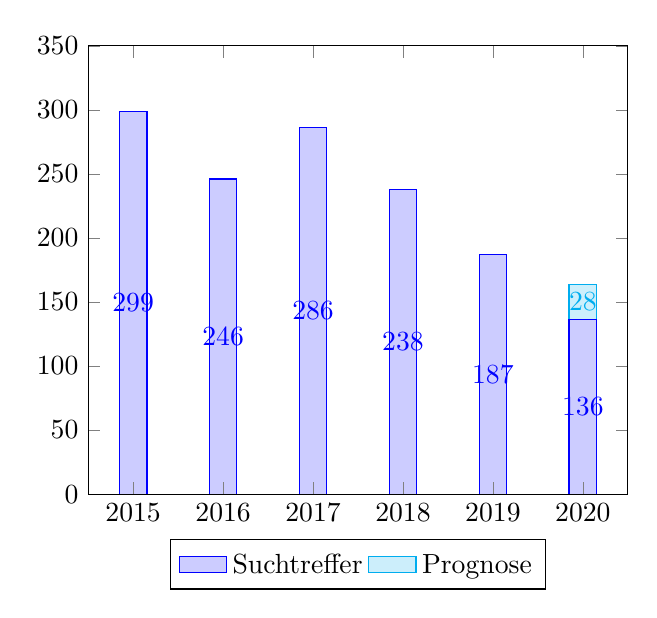
\begin{tikzpicture}
	\begin{axis}[
		ybar stacked,
        ymin=0,
        ymax=350,
        ytick distance={50},
		area style,
		legend style={at={(0.5,-0.10)},anchor=north,legend columns=-1},
		nodes near coords,
		symbolic x coords = {2015, 2016, 2017, 2018, 2019, 2020},
	]
		\addplot+[blue,fill opacity=0.2,text opacity=1,ybar,no marks]
			plot coordinates {
			(2015,299)
			(2016,246)
			(2017,286)
			(2018,238)
			(2019,187)
			(2020,136)
			};
		\addplot+[cyan,fill opacity=0.2,text opacity=1,ybar,no marks]
			plot coordinates {
			(2015,0)
			(2016,0)
			(2017,0)
			(2018,0)
			(2019,0)
			(2020,28)
			};
		\legend{\strut Suchtreffer, \strut Prognose}
	\end{axis}
\end{tikzpicture}
\caption{Studien zur Browserkompatibilität, eigene Darstellung (vgl. \ref{sec:studien-zur-browser-kompatibilitaet})}
\label{fig:studien-zur-browser-kompatibilitaet}
\end{wrapfigure}

Die Vielfalt an Browsern bereitet Webentwicklern immer wieder eine Herausforderung, dass ein von ihnen bereitgestelltes Produkt für die Nutzer einwandfrei funktioniert, unabhängig ihrer Browserpräferenz. Die Häufigkeit solcher Probleme, auch Cross-Browser-Incompatabilities (XIB) genannt, hat jedoch durch einen abgenommen, unter anderem erklärbar durch den Trend von offenen Web-Standards \cite{W3CStandards}.

Generell lässt sich feststellen, dass auch in der Literatur die Veröffentlichungen in Bezug auf (In-)Kompatibilität von Browsern abnimmt, dies ist in \autoref{fig:studien-zur-browser-kompatibilitaet} zu betrachten. Was dafür spricht, dass das Problem nicht mehr so präsent ist, wie zuvor.

Im Jahr 2020 gab es weitere Entwicklungen, die die Kompatibilität zwischen Browsern erhöhte. Microsoft hat beim Folgeprodukt zum Internet Explorer, den Microsoft Edge Browser, von einer proprietären Browserengine zu Chromium gewechselt \cite{MicrosoftEdgeChromium} und enthält somit den selben Kern wie Chrome und Opera. Zum Ende 2020 wird zudem der Support für den Internet Explorer 11 eingestellt \cite{MicrosoftInternetExplorerDeprecation}. Zum September 2020 meldete Statista eine Marktverteilung von 69,71\% Chrome, 8,73\% Safari, 8,15\% Firefox, 5,54\% Edge, 2,51\% Internet Explorer und 2,3\% Opera \cite{StatistaBrowserMarketshare}.

\subsection{JavaScript}

Als JavaScript 1997 veröffentlicht und in den NetScape Navigator integriert wurde, gab es die berechtigen Bedenken, dass das Öffnen einer Webseite dem Betreiber erlaubt Code auf dem System eines Nutzers auszuführen. Damit dies nicht eintritt, wurde der JavaScript Ausführungskontext in eine virtuelle Umgebung integriert, einer Sandbox. \cite{LearningJavaScript}

Die JavaScript-Sandbox bei Browsern schränkt ein, dass unter anderem kein Zugriff auf das Dateisystem erfolgen kann. Auch Zugriff auf native Bibliotheken oder Ausführung von nativem Code ist nicht möglich \cite{TheSpyInTheSandbox}. Browser bieten dafür aber einige Schnittstellen an, die es erlauben z. B. Daten beim Client zu speichern oder auch Videos abzuspielen.

\nomenclature[Fachbegriff]{CORS}{Cross-Origin Resource Sharing}
\nomenclature[Fachbegriff]{Ajax}{Asynchronous JavaScript and XML}
\nomenclature[Fachbegriff]{W3C}{World Wide Web Consortium}
\nomenclature[Fachbegriff]{XHR}{XMLHttpRequest}

Microsoft nahm 1999 im Internet Explorer 5.0 eine neue Methode in ihre JavaScript-Umgebung auf, um den Funktionsumfang zu erweitern: Ajax (Asynchronous JavaScript and XML). Ajax erlaubt die Datenabfrage von Webservern mittels JavaScript. Hierdurch wird ermöglicht, dass Inhalte auf Webseiten dynamisch abgefragt und dargestellt wurden, zuvor war hierfür ein erneuter Seitenaufruf notwendig. Das Konzept wurde kurz darauf von allen damals gängigen Browser übernommen. Erst jedoch mit der Standardisierung 2006 durch das W3C \cite{TheXMLHttpRequestObject} fand die Methode Anklang und Einsatz bei Entwicklern und ist seitdem der Grundstein für unser dynamisches und interaktives Web \cite{TheStoryOfXMLHTTP}.

Webapplikationen wurden nun immer beliebter, aber Entwickler klagten darüber, dass Browser die Abfragen von JavaScript nur auf dem bereitstellenden Webserver, also ``same-origin``, erlauben\cite{CrossSiteXHRWithCORS}. Im selben Jahr der Standardisierung von Ajax, wurde ein erster Entwurf zur Ermöglichung und Absicherung von Abrufen domänenfremder Ressourcen eingereicht \cite{AuthorizingCORS}, das sogenannte Cross-Origin Resource Sharing.

% {\color{red}\textit{TODO: add some more which flows into the next subsection}}

Im folgenden Abschnitt werden, für diese Arbeit relevante, Sicherheitsvorkehrungen von Browsern vorgestellt und beschrieben - darunter auch Cross-Origin Resource Sharing.

%\subsubsection{Fehleranfälligkeit}
%
%Die Sprache JavaScript stellt an sich auch eine Besonderheit der Umgebung dar. Denn anders als z. B. C, C++, Java gilt sie als fehleranfällig \cite{FastReproducingWebApplicationErrors}. Dies

\subsection{Sicherheitsvorkehrungen}

% Zusätzlich zu der Sandbox gibt es weitere Vorkehrungen, die definieren welche Daten innerhalb der JavaScript Umgebung abgerufen und mit welchen Diensten kommuniziert werden darf \cite{LearningJavaScript}. Zwei wichtige dieser Vorkehrungen, die eine Webapplikationen nutzen kann bzw. beachten muss, werden folgend erklärt.

\subsubsection{Cross-Origin Resource Sharing (CORS)}

Das Konzept von CORS stellt sicher, dass aus einer JavaScript-Umgebung heraus keine Ressourcen von Webservern angefragt werden, außer diese Webserver stimmen der Anfrage zu \cite{MDNCORS}. Folgendes vereinfachtes Beispiel soll den Nutzen und den generellen Ablauf von CORS näher erläutern:

\begin{quotation}
Ein Nutzer ruft eine Webapplikation auf, welche unter \texttt{localhost:3000} bereitgestellt wird. Diese Webapplikation sendet, für den Nutzer unwissend, Anfragen an einen Facebook Dienst. Dies lässt der Browser aber nur zu, wenn der Dienst von Facebook explizit bestätigt, dass eine Anfrage von \texttt{localhost:3000} diese Aktion ausführen darf.

Dafür sendet der Browser eine OPTIONS-Anfrage, in der die Herkunft (``Origin``) der Anfrage notiert ist. Der Facebook Dienst antwortet daraufhin mit den entsprechenden CORS-Headern und gibt somit an, ob die Anfrage von dieser Origin aus erlaubt ist. Nun prüft der Browser, ob die von Facebook übermittelten Origins übereinstimmen. Ist dies nicht der Fall, wird die Anfrage im Browser blockiert und im JavaScript Kontext schlägt dieser fehl. Details zum Fehler werden der JavaScript-Umgebung bewusst enthalten.
\end{quotation}

\subsubsection{Content-Security-Policy}

\nomenclature[Fachbegriff]{CSP}{Content-Security-Policy}
\nomenclature[Fachbegriff]{XSS}{Cross-Site-Scripting}
\nomenclature[Fachbegriff]{CDN}{Content Delivery Network}

Eine Content-Security-Policy (CSP) definiert, welche Funktionalitäten einer Webapplikation aus geladen zur Verfügung stehen. Dies dient unter anderem dem Schutz vor Cross-Site-Scripting, indem eine Webapplikation beschränken kann, welche Funktionalitäten in JavaScript verfügbar sind und von wo aus JavaScript und CSS Skripte geladen werden dürfen \cite{MDNContentSecurityPolicy}. Weiterhin kann bei einem Versuch der Webapplikation die Regeln zu umgehen Bericht darüber erstattet werden.

%Nachfolgendes Beispiel soll den Nutzen etwas näher bringen:

%\begin{quotation}
%Eine Webapplikation, welche zwei numerische Eingaben von einem Nutzer entgegennimmt und darauf basierend eine komplexe Operation ausführt und das Ergebnis anzeigt. Diese Operation wird über ein eingebundenes Skript von einem CDN bereitgestellt. Weiterhin wird die Datenverarbeitung über ein eigens bereitgestelltes Skript durchgeführt. Da wir unseren Anwendungsfall kennen, kann durch die Härtungsmaßnahme einer CSP die Webapplikation abgesichert werden. Hierfür werden die Funktionalitäten auf das Folgende beschränkt:
%
%\begin{itemize}
%	\item Das Laden von JavaScript vom eigenen Webserver (\textbf{self}) und vom CDN.
%	\item Das Laden von \texttt{inline}-Skripten wird nicht erlaubt (und ist damit verboten).
%	\item Bei Verstoß soll ein Bericht an einen eigenen Protokollserver gesendet werden.
%\end{itemize}
%
%Die entsprechende CSP sieht wie folgt aus:
%
%\begin{verbatim}
%Content-Security-Policy: default-src 'self'; script-src 'self' example.com;
%\end{verbatim}
%
%Wird nun das Skript des CDN kompromittiert und versucht 
%\end{quotation}

\subsection{Logdaten}

Ähnlich wie bei anderen Umgebungen gibt es eine standardisierte Log- bzw. Konsolenausgabe für die JavaScript Umgebung \cite{MDNConsole}. Diese Ausgabe ist aber für den Standard-Benutzer eher unbekannt und der Zugriff darauf sowie die Funktionen dessen können je nach Browser variieren. Deswegen kann in den meisten Fällen nicht darauf gehofft werden, dass die Nutzer dieses Log bereitstellen. Zusätzlich ist es durch die zuvor beschrieben Härtungsmaßnahmen von Browsern nicht möglich das Log in eine Datei zu schreiben.

Eine Automatisierung der Logdatenerhebung ist zudem auch nicht trivial, denn die Daten, welche in die Ausgabe geschrieben werden, sind nicht aus der JavaScript Umgebung aus lesbar. Alternativ können die Daten selber erhoben oder abgefangen werden. Hierbei besteht aber weiterhin die Hürde, wie die Daten an die Stakeholder gelangen.

\subsection{Fernzugriff}

Ein weiterer Punkt, der die Umgebung ``Browser`` von anderen unterscheidet, ist dass die Stakeholder sich normalerweise nicht auf die Systeme der Nutzer schalten können. Bei Expertenanwendungen ginge dies vielleicht, aber wenn eine Webapplikation für den offenen Markt geschaffen ist, sind die Nutzer zahlreich und unbekannt.

Weiterhin gibt es standardmäßig keine Funktionalität wie z. B. das Remote Application Debugging \cite{JavaDebugWireProtocol}, welches Java unterstützt.
